%%%%%%%%%%%%%%%%%%%%%%% file template.tex %%%%%%%%%%%%%%%%%%%%%%%%%
%
% This is a general template file for the LaTeX package SVJour3
% for Springer journals.          Springer Heidelberg 2010/09/16
%
% Copy it to a new file with a new name and use it as the basis
% for your article. Delete % signs as needed.
%
% This template includes a few options for different layouts and
% content for various journals. Please consult a previous issue of
% your journal as needed.
%
%%%%%%%%%%%%%%%%%%%%%%%%%%%%%%%%%%%%%%%%%%%%%%%%%%%%%%%%%%%%%%%%%%%

\RequirePackage{fix-cm}
%
\documentclass{svjour3}                     % onecolumn (standard format)
%\documentclass[smallcondensed]{svjour3}     % onecolumn (ditto)
%\documentclass[smallextended]{svjour3}       % onecolumn (second format)
%\documentclass[twocolumn]{svjour3}          % twocolumn
%
\smartqed  % flush right qed marks, e.g. at end of proof
%
\usepackage{graphicx}
\usepackage[numbers]{natbib}
\usepackage{hyperref}

\begin{document}

\title{Particle streak velocimetry using Ensemble Convolutional Neural Networks}
\titlerunning{Streaks imaging with CNN}        % if too long for running head

\author{Alexander V. Grayver         \and
        Jerome Noir
}

\institute{A. V. Grayver \at
              Institute of Geophysics, ETH Zurich \\
              Sonneggstrasse 5 \\
							8092 Zurich, Switzerland \\
              Tel.: +41-44-6333154\\
              \email{agrayver@erdw.ethz.ch}
              \and
           J. Noir \at
					    Institute of Geophysics, ETH Zurich \\
              Sonneggstrasse 5 \\
							8092 Zurich, Switzerland \\
              Tel.: +41-44-6337593\\
              \email{jerome.noir@erdw.ethz.ch}
}

\date{Received: - / Accepted: -}


\maketitle

\begin{abstract}
Insert your abstract here. 
\keywords{Streak analysis \and Neural Networks \and Turbulent Flow}
\end{abstract}

\section{Introduction}
\label{sec:intro}

Particle Image Velocimetry (PIV) is arguably the most widely used technique to quantitatively study experimental flows \cite{raffel2018particle}. A common work-flow would consist of seeding flow with luminescent particles and taking pairs of pictures with a known short time separation to capture an instantaneous flow state. By splitting a pair of images into (possibly overlapping) windows and cross-correlating between them allows one to infer the direction and magnitude of the flow. With modern computers and digital cameras, PIV has experienced wide adoption in the scientific community \textbf{add refs}. For cross-correlation to work properly, one has to ensure that the exposure time is short enough such that particles do not move more than a few pixels and the two images have clearly identifiable correlations, thus the mean motion has to remain predominantly linear. Violating this condition, for instance because of insufficient laser intensity or too fast flow, results in so called streaks - traces of particles.

Streaks in the PIV images are commonly considered an experimental failure since they render cross-correlation techniques less efficient or even inapplicable. When flow velocity imposes constraints for which the camera and light source at hand cannot capture steady particles, one either has to use a higher speed camera or/and a stronger light source. Both of these solutions quickly hit financial and safety constraints, which often cannot be overcome in academia. Although not suitable for conventional cross-correlation methods, streak images do contain information about the flow. A Even though an image with streaks does not contain information about direction of the underlying flow, information on the mean velocity magnitude and azimuth can be inferred from streaks themselves. To the best of authors' knowledge, there have been no attempts to do this before, which motivated us to design a method for extracting information about the flow from streaks. 

To this end, we applied an ensemble of Convolutional Neural Networks (CNN) trained on streak images to draw a statistical prediction of the displacement magnitude and corresponding azimuth. The potential of CNNs has long been recognized for applications related to the face and handwriting recognition \cite{lawrence1997face, simard2003best}, although their power has been fully discovered only recently when deeper (that is, with more layers) networks became feasible to train within reasonable amount of time, mostly due to emerge of Graphic Processor Units (GPUs) \cite{krizhevsky2012imagenet, karpathy2014large}. An interested reader is referred to a recent overview of the deep learning with important development milestones listed \cite{lecun2015deep}.

Before we proceed to describing methodology and results, it is worth to mention that a crucial ingredient to a success of CNNs is a suitably large training set, which a CNN is supposed to learn from without facing an over-fitting. From this perspective, streak analysis appears almost an ideal problem. Similar to PIV, we make a reasonable assumption that within a sufficiently small interrogation window velocity exhibits simple functional form (for instance, constant or linear function). This allows us to quickly generate an unlimited number of training images. Adding variability in number of streaks per window, their thickness and intensity will well mimic a realistic experimental scenario. Therefore, we can exhaustively sample the parameter space and feed the network with as many sample as needed to attain an acceptable accuracy. The specific numbers and parameters will be discussed in the corresponding sections below.

\section{Methods}
\label{sec:methodology}

\subsection{Problem setup}

We aim at inferring the displacement and azimuth from a gray scale image of size $n \times n$ pixels depicting streaks (Figure \ref{fig:fig1}). In real settings, these images are excerpts (obtained, for instance, after applying a sliding window) of a larger $N \times N$ pixels image taken by a camera. For purposes of our experiments, we chose $n = 48$, but the approach presented below is general. We assume that within $n \times n$ window, the velocity is a constant, thus streaks have the same length and direction with small variations, treated as noise. In contrast, the number of streaks ($[2, 10]$), their color intensity ($[200, 255]$, where 0 is black and 255 is white) and thickness ($[2, 4]$ pixels) vary. Additionally, streaks are allowed to go outside the image, which is often the case in real settings, thus a CNN is supposed to be resilient to such cases. Once streaks are generated, they are blurred with a Gaussian kernel of $3\times 3$ pixels. The maximum displacement, $r_\textnormal{max}$, of a particle within an image is assumed to be half of the chosen window size, that is $r_\textnormal{max} = 24$ pixels in our case. Each streak is thus characterized by two numbers $\Delta, \phi$, denoting displacement and azimuth, respectively. 

To generate train and validation images, we sampled $\Delta$ and $\phi$ from the uniform distributions
\begin{equation}
\Delta \sim U(1, r_\textnormal{max}) 
\end{equation}
and
\begin{equation}
\phi \sim U(-\pi/2+\delta, \pi/2),
\end{equation}
respectively. 
%This choice ensures that we sample a half-circle of radius $r_\textnormal{max}$ uniformly. 
Here, $\phi = 0$ corresponds to the positive $x$-axis and increases clockwise. 
Note that limits for $\phi$ cover only half of the circle minus $\delta = 5^{\circ}$ on one end to avoid ambiguity with respect to the direction. Figure \ref{fig:fig1} shows a selection of streak images generated using the stated procedure. The outlined procedure enables generation of millions of images in just a few minutes on a regular PC. 

\begin{figure}
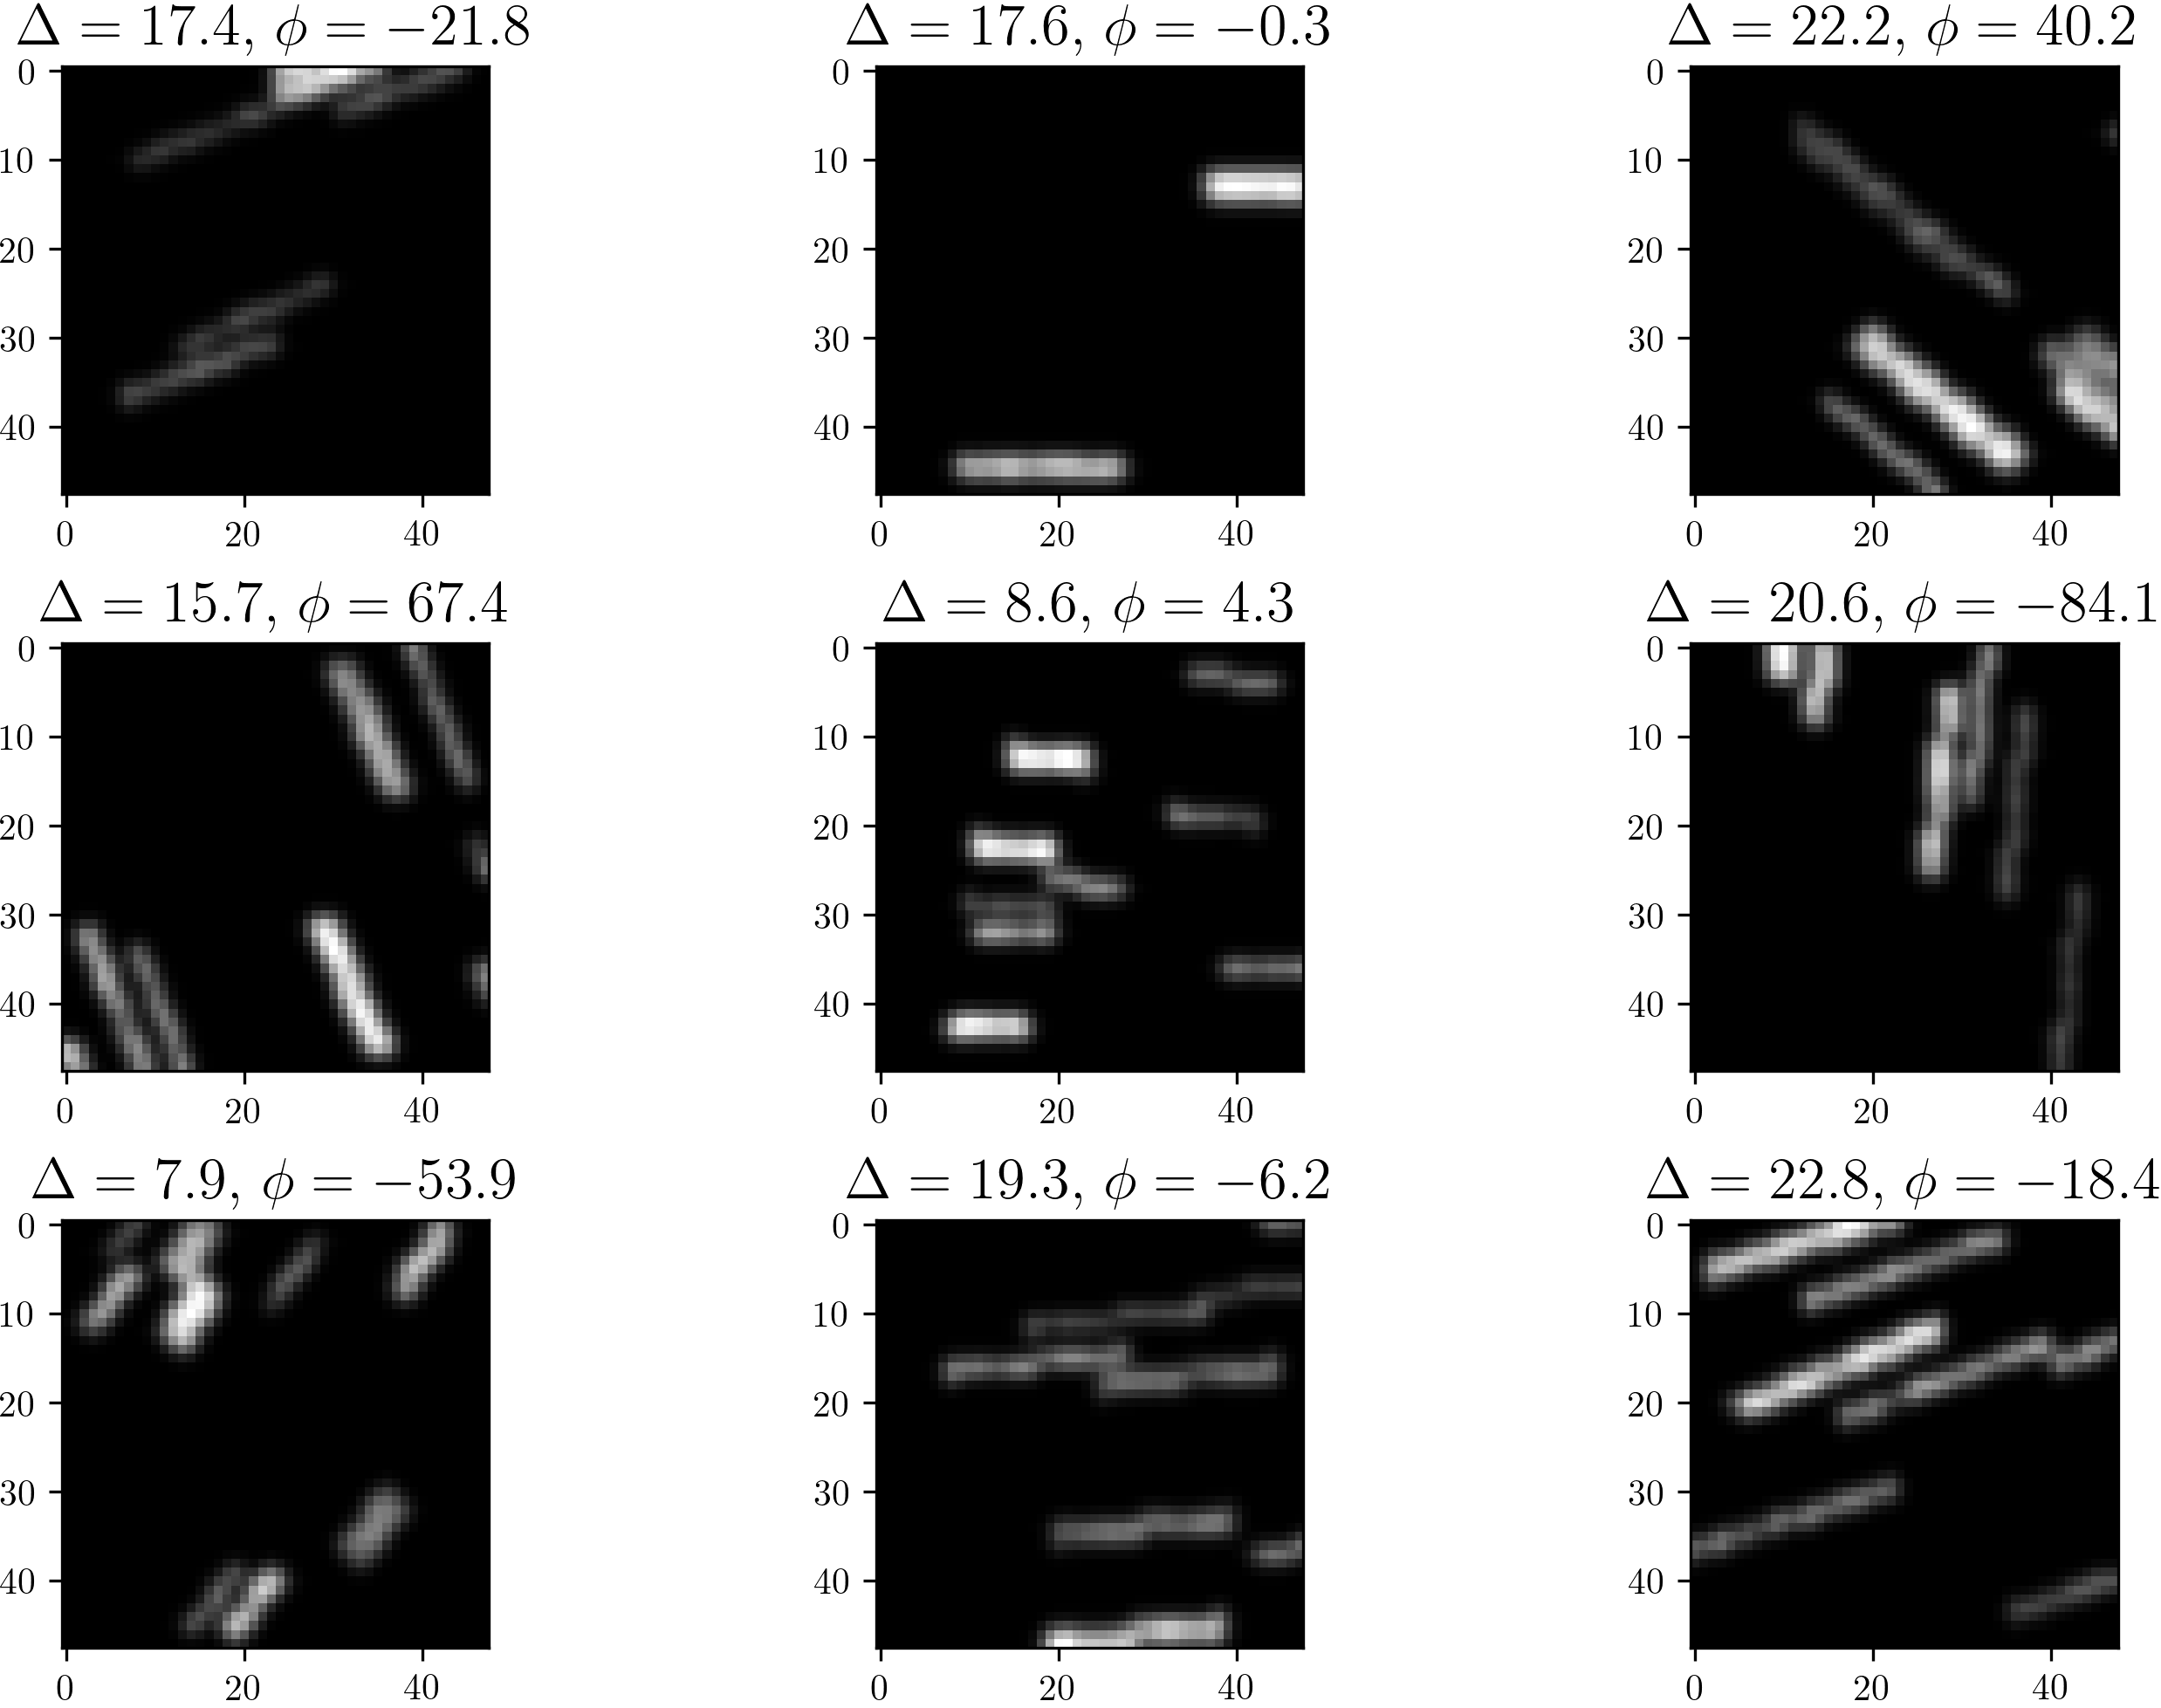
\includegraphics[width=\textwidth]{figs/figure1.png}
\caption{Subset of generated streak images used for training and validation with corresponding displacements (in pixels) and azimuth angles (in degrees) given in titles.}
\label{fig:fig1}
\end{figure}

\subsection{Network architecture and implementation}

Whereas there may exist more efficient architectures, we found that for our problem increasing depth of the network has not improved overall performance significantly, nor did increasing and/or decreasing filter size. Additionally, we found that, in contrast to majority of reported CNN architectures, using the average pooling instead of the max pooling results in higher accuracy.

To prevent overfitting and improve representative power of the network, we added batch normalization at the end of each convolution unit \cite{ioffe2015batch} and dropout with the 30\% drop fraction \cite{srivastava2014dropout}.

\begin{figure}
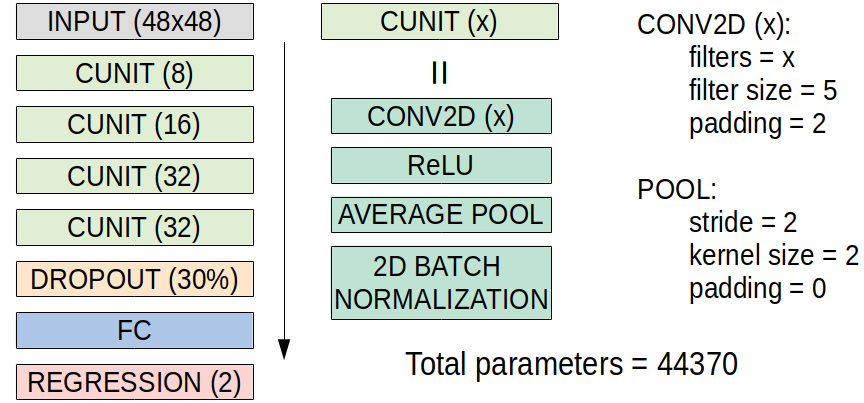
\includegraphics[width=\textwidth]{figs/figure_CNN.png}
\caption{Architecture of the network. Left: sequence of layers and corresponding parameters in the brackets. Each CUNIT layer consists of four actual layers listed in the middle column. Relevant layer parameters are given on the right. Total number of learnable parameters in the network is 44370.}
\label{fig:fig2}
\end{figure}

To increase accuracy and robustness of the prediction \cite{hinton2015distilling}, we trained an ensemble consisting of ten networks. All networks have identical architecture and parameters, but were trained using different randomly chosen initial weights \cite{glorot2010understanding, he2015delving} and shuffled batches, thus forming a unique sequence of batches supplied to the ADAM optimizer. The outputs of all models are averaged to geta the final prediction.

Finally, the network was implemented using the PyTorch library. The complete implementation can be found using the link below.

\section{Results}

\subsection{Network accuracy}

\subsection{Validation with DNS}

\subsection{Validation with experimental images}

\section{Conclusions}

Extension: non-constant velocity (polynomials -> more output variables and possibly deeper network).
Streak localization and tracking: more complex architectures.

\begin{acknowledgements}
We thank authors of PyTorch, mathplotlib and h5py python packages for making them available, Meredith Plumley for sharing her DNS data, Adrian Tasistro-Hart for a number of insightful discussions on CNNs. The Juoyter Python notebooks of all programs used in this study can be found here \url{https://github.com/agrayver/streakcnn}.
\end{acknowledgements}


% References
%\bibliographystyle{spbasic}      % basic style, author-year citations
\bibliographystyle{spmpsci}      % mathematics and physical sciences
%\bibliographystyle{spphys}       % APS-like style for physics
\bibliography{refs}

% Non-BibTeX users please use
%\begin{thebibliography}{}

%\end{thebibliography}

\end{document}
